% !TEX root = ../main.tex

\section{Results}

\subsection{\ref{rq:disp}: Dispersion accross tasks and proficiency levels}

To examine the evenness of occurrence of second conditionals across tasks and proficiency levels, I calculated dispersion indices ($DP$ and $DP_{norm}$) using different definitions of corpus “parts”. 
First, I partitioned the data into the 20 task topics. Second, the data was divided by proficiency level (lower vs. higher). 
Finally, I calculated topic dispersion separately within each proficiency group. 
Table \ref{tab:dispersion} reports $DP_{norm}$, since raw $DP$ values are nearly identical.

\begin{table}[htbp]
\centering
\begin{tabular}{lc}
\hline
\textbf{Partitioning / subset condition} & \textbf{DP\textsubscript{norm}} \\
\hline
Topics across all data & 0.559 \\
Proficiency level as partitioning variable & 0.022 \\
\hline
\textit{Topic dispersion within proficiency groups} & \\
Low proficiency (topics) & 0.182 \\
High proficiency (topics) & 0.376 \\
\hline
\end{tabular}
\caption{Dispersion of type II conditionals. The last block shows topic dispersion calculated separately for low- and high-proficiency subsets.}
\label{tab:dispersion}
\end{table}

Overall, dispersion across task topics was relatively high, suggesting that different tasks elicited considerably different numbers of type II conditionals in their responses.
Nevertheless, when stratifying the tasks by proficiency levels, higher-level tasks showed a more uneven dispersion than lower-level ones.
On the other hand, dispersion across levels was very low, revealing that both proficiency groups produced a very similar number of conditionals to what would be expected by their corresponding size.

\begin{figure}[htbp]
    \centering
    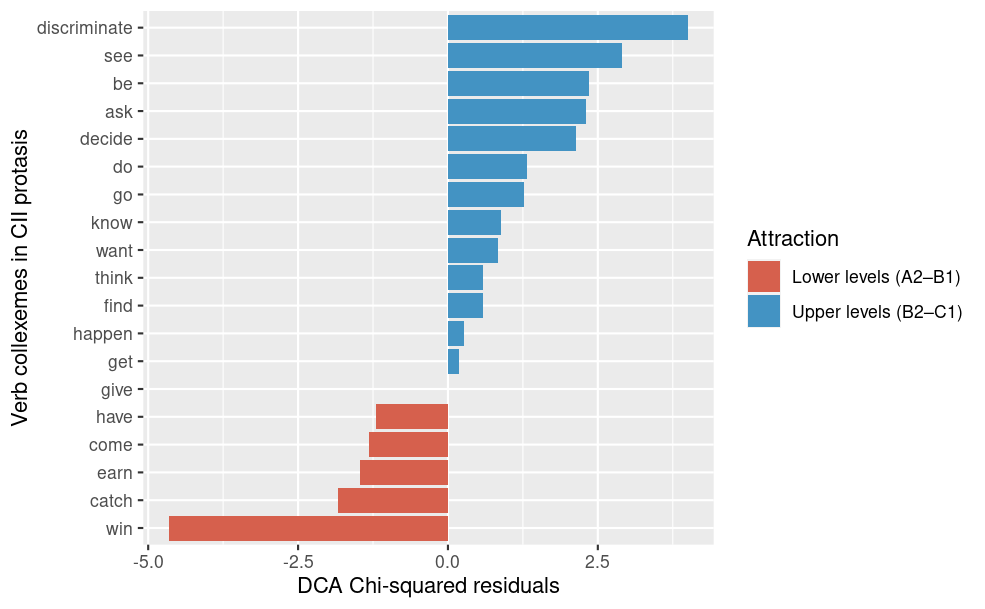
\includegraphics[width=0.7\textwidth]{images/Residuals.png}
    \caption{Residuals of the $\chi^{2}$-test}
    \label{fig:residuals}
\end{figure}


\subsection{\ref{rq:lexical_div}: Lexical diversity in protasis verbs}

